


\begin{tikzpicture}[y=0.80pt, x=0.8pt,yscale=-1, inner sep=0pt, outer sep=0pt]
  \path[draw=black,miter limit=4.00,line width=1.200pt]
    (15.2615,55.3504)arc(260.000:290.000:200.051);
  \path[draw=black,line join=round,miter limit=4.00,line width=1.200pt]
    (6.4976,5.6478)arc(260.000:290.000:250.520);
  \path[draw=black,dash pattern=on 2.40pt off 0.80pt,line join=round,miter
    limit=4.00,line width=0.800pt] (11.7974,30.7804)arc(260.000:290.000:220.000000
    and 225.000);
  \path[draw=black,line join=miter,line cap=butt,line width=0.800pt]
    (20.0000,82.3622) -- (10.0000,32.3622);
  \path[draw=black,line join=miter,line cap=butt,line width=0.800pt]
    (120.0000,63.3622) -- (136.0000,19.3622);
  \path[draw=black,line join=miter,line cap=butt,line width=0.800pt]
    (50.0000,27.3622) -- (35.0000,52.3622) -- (50.0000,52.3622) --
    (50.0000,2.3622) -- (65.0000,2.3622) -- cycle;
  \path[draw=black,line join=miter,line cap=butt,line width=0.800pt]
    (205.0000,27.3622) -- (190.0000,52.3622) -- (205.0000,52.3622) --
    (205.0000,2.3622) -- (220.0000,2.3622) -- cycle;
  \path[draw=black,line join=round,miter limit=4.00,line width=0.400pt]
    (320.0000,2.3622) .. controls (303.3333,6.5288) and (290.8333,10.6955) ..
    (282.5000,14.8622) .. controls (274.1667,19.0288) and (270.0000,23.1955) ..
    (270.0000,27.3622) .. controls (270.0000,31.5288) and (274.1667,35.6955) ..
    (282.5000,39.8622) .. controls (290.8333,44.0288) and (303.3333,48.1955) ..
    (320.0000,52.3622);
  \path[draw=black,line join=miter,line cap=butt,miter limit=4.00,line
    width=0.400pt] (270.0000,-2.6378) -- (270.0000,57.3622);
  \path[rounded corners=0.0000cm] (270.0000,2.3622) rectangle (320.0000,52.3622);
  \path[draw=black,line join=round,miter limit=4.00,nonzero rule,line
    width=0.036pt] (270.2687,13.6105) -- (270.2687,2.6241) -- (293.9518,2.6312) ..
    controls (306.9774,2.6350) and (317.5946,2.6541) .. (317.5455,2.6734) ..
    controls (317.4964,2.6928) and (316.5321,2.9481) .. (315.4026,3.2408) ..
    controls (306.5721,5.5288) and (297.6297,8.3134) .. (291.2062,10.7754) ..
    controls (285.3657,13.0139) and (280.1754,15.5360) .. (276.8759,17.7389) ..
    controls (273.8601,19.7523) and (271.6927,21.8931) .. (270.6331,23.9051) --
    (270.2687,24.5969) -- (270.2687,13.6105) -- cycle;
  \path[draw=black,line join=round,miter limit=4.00,nonzero rule,line
    width=0.036pt] (270.2700,41.1286) -- (270.2710,30.1688) -- (270.6355,30.8384)
    .. controls (271.2381,31.9454) and (271.7596,32.6102) .. (272.9854,33.8335) ..
    controls (274.1743,35.0201) and (275.0062,35.7060) .. (276.5185,36.7462) ..
    controls (283.5625,41.5917) and (296.6443,46.5481) .. (315.4917,51.5123) --
    (317.6345,52.0767) -- (293.9515,52.0826) -- (270.2685,52.0885) --
    (270.2695,41.1286) -- cycle;
  \path[draw=black,dash pattern=on 2.40pt off 2.40pt,line join=miter,line
    cap=butt,miter limit=4.00,line width=0.800pt] (25.0000,107.3622) --
    (20.0000,82.3622);
  \path[fill=black] (29.7995,97.515488) node[above right] (text8240) {\(\rho =
    \sfrac{-1}{\kappa}\)};
  \path[fill=black] (140,52.362183) node[above right] (text8244) {\(t\)};
  \path[fill=black] (30,67.362183) node[above right] (text8248) {\(\epsilon = -y
    \kappa\)};
  \path[fill=black] (180,67.362183) node[above right] (text8252) {\(\sigma =
    E\epsilon\)};
  \path[fill=black] (265,67.362183) node[above right] (text8256) {\(dM = y \sigma
    dA\)};
  \path[fill=black] (225,2.3621817) node[above right] (text8500) {\(y =
    \sfrac{t}{2}\)};
  \path[draw=black,line join=miter,line cap=butt,miter limit=4.00,line
    width=0.400pt] (205.0000,-2.6378) -- (205.0000,57.3622);
  \path[fill=black] (215,52.362183) node[above right] (text8506) {\(y =
    -\sfrac{t}{2}\)};

\end{tikzpicture}

